\section{Introduction}
\label{sec:introduction}
%TODO in each section mention research gaps

\subsection{Tropical forest}
	\begin{figure}[ht]
		\centering
		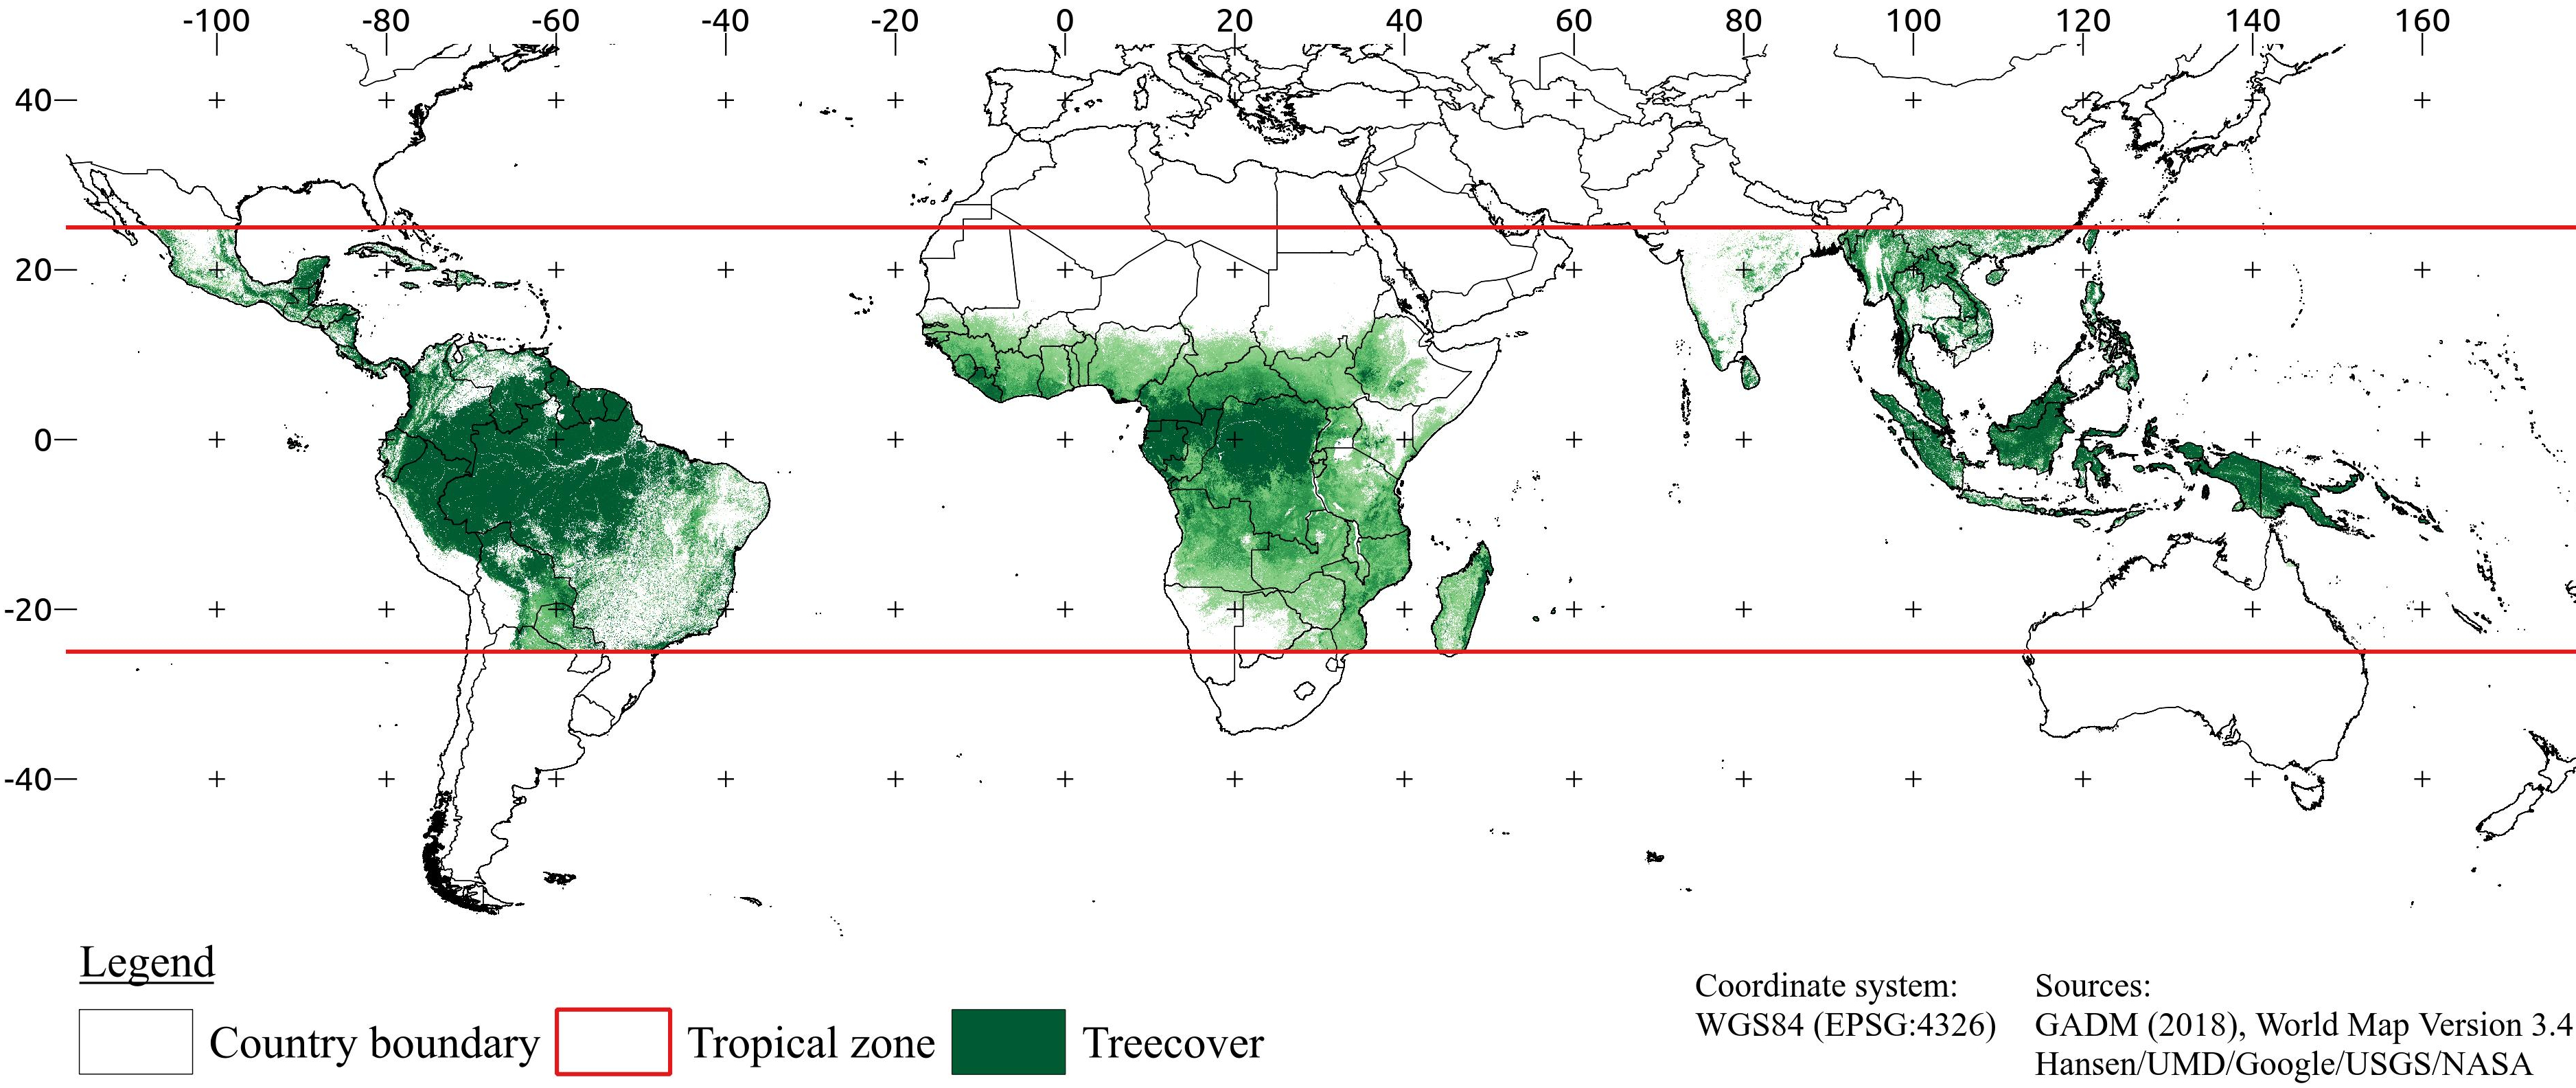
\includegraphics[scale=0.97]{img/intro_overview_frameless}
		\caption[Tropical zone]{Geographic tropical zone framed red and the tropical forest}
		\label{fig:tropicalzone}
	\end{figure}

	\subsubsection{Current state}
	\subsubsection{Contribution to climate}
	\subsubsection{Forest definitions}

\subsection{Deforestation}
	\begin{figure}[ht]
		\centering
		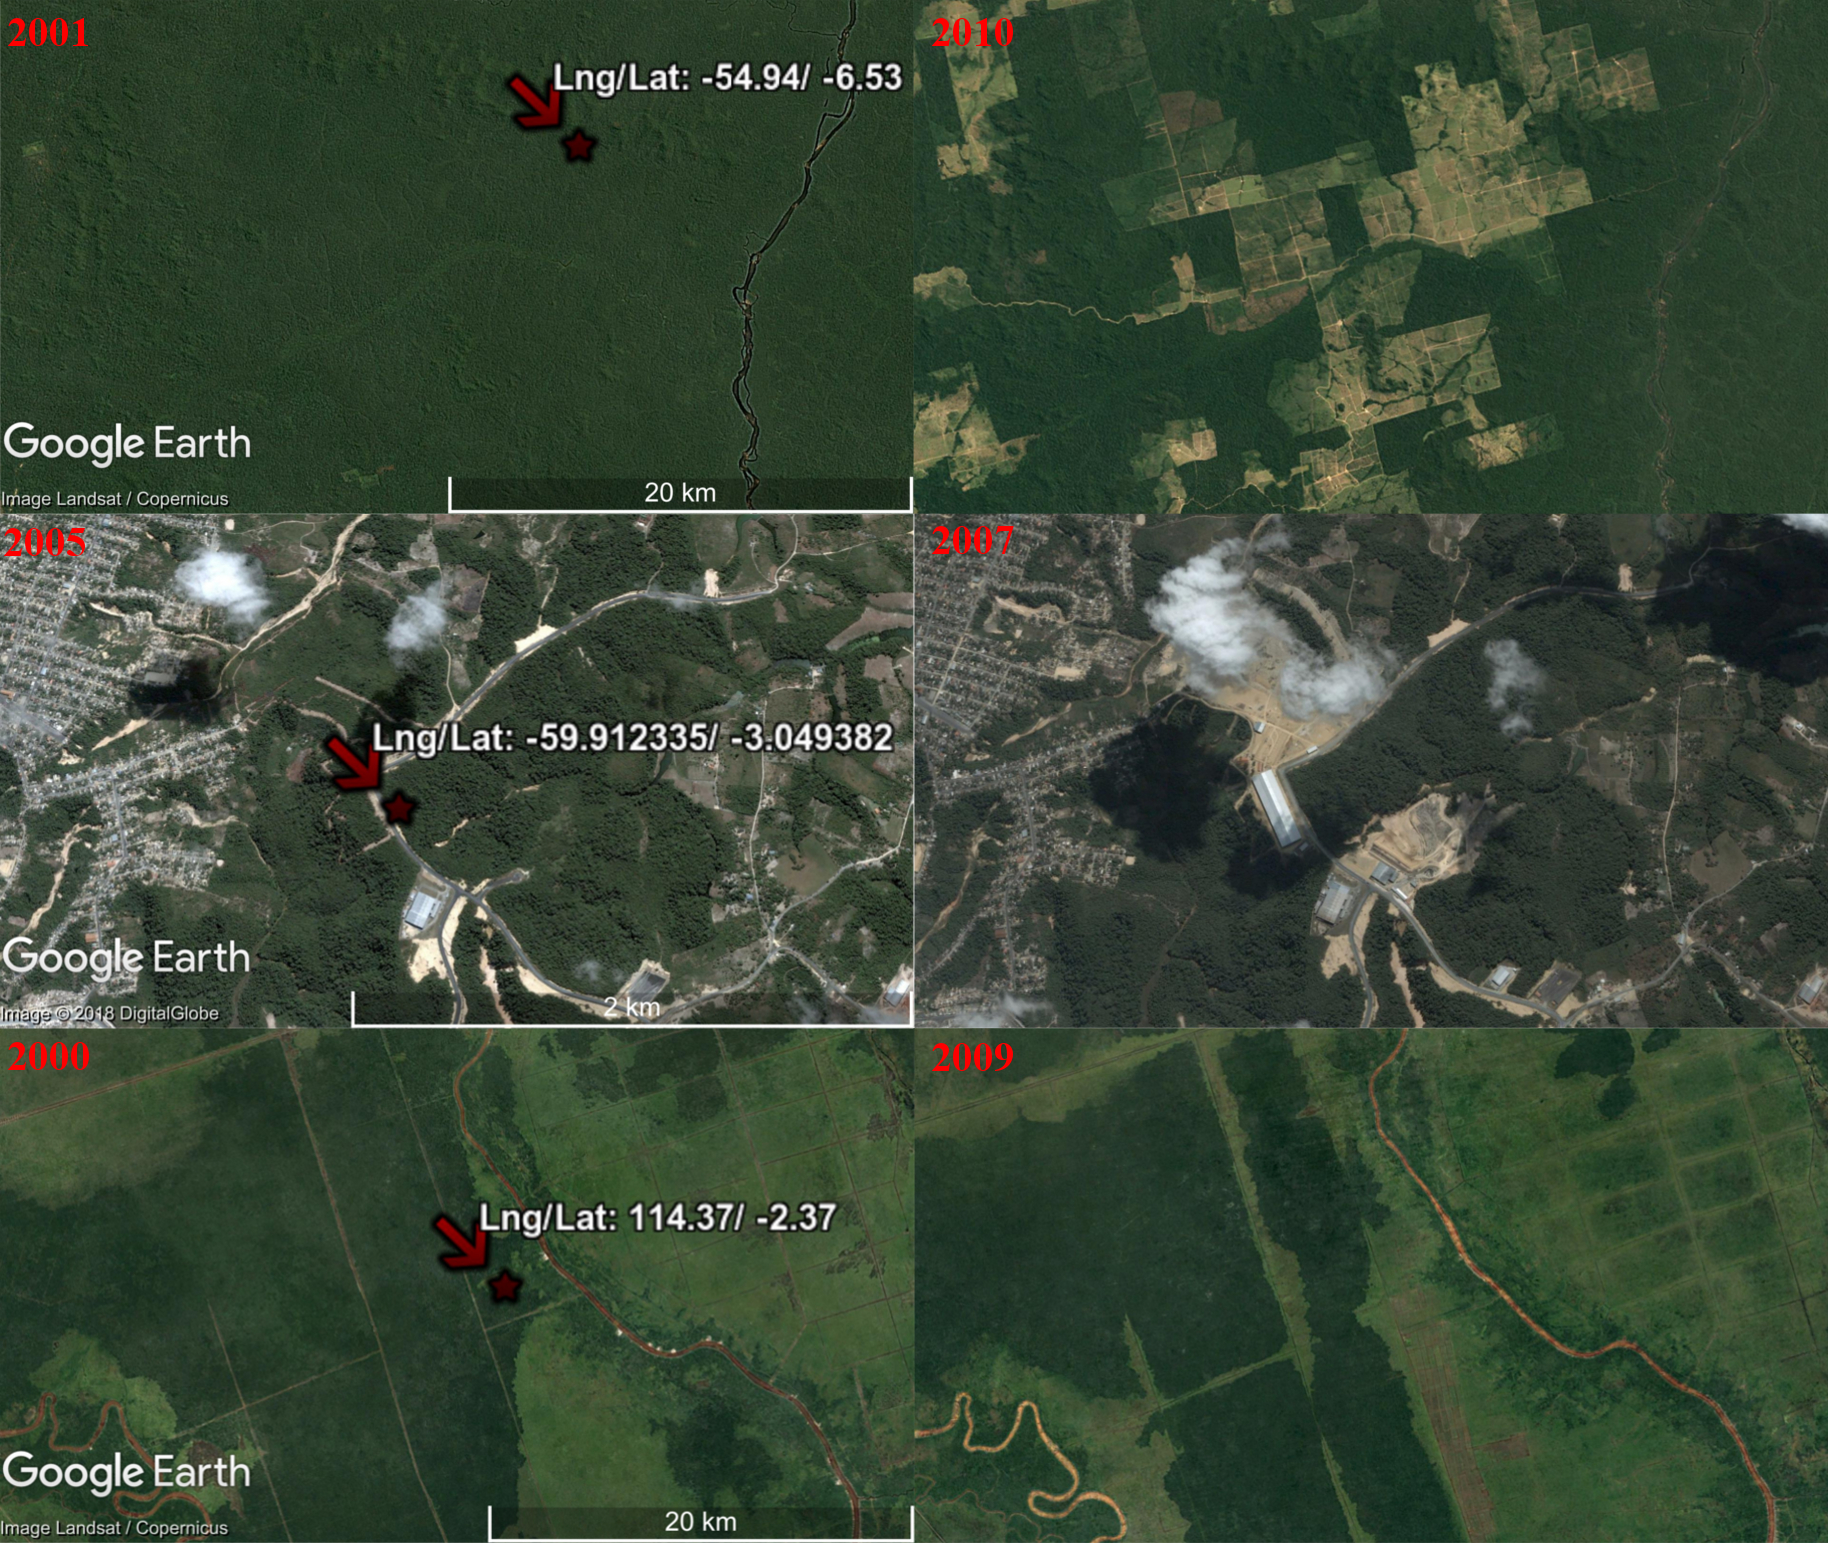
\includegraphics[scale=0.6]{img/deforestation_examples}
		\caption[Deforestation examples]{Upper Brazil agriculture, middle Brazil urbanization, lower Indonesia large scale palm oil plantations}
		\label{fig:deforestationexamples}
	\end{figure}

	{\color{red} Gaps no spatial explicit knowledge on direct deforestation drivers (amount, pattern, cattle ranching/cropland, urbanization)}
	{\color{red} Contribution of deforestation drivers on ghg emissions, no knowledge on soil organic carbon emissions}
 
	\subsubsection{Land use and land cover change}
	\subsubsection{Drivers of deforestation}
	\subsection{Emissions trough deforestation}
	\subsubsection{Removal of AGB}
	\subsubsection{Soil organic carbon change and soil dynamics}

\subsection{Ecosystem services}
	{\color{red} till now only estimates of losses no balance estimate} 
	\subsubsection{Ecosystem service values}
	\subsection{Research objective and questions}
